\chapter{Medical imaging techniques}
\label{sec:chap3}

\section{X-Ray \& CT Imaging}
X-ray is one of the early modules introduced by Wilhelm Rontgen. With this modality, we could look within the body without having to cut the body. Another modality that goes along with x-ray is computed tomography (CT). Computed tomography allows you to look into the 3D projection of every single part of the body and create visual anatomy of the body.

The first part is on x-ray generations and how it works. We have something called an \textbf{x-ray tube}, and this is the source of generated x-ray. It is not an optical photon, i.e., unlike LED lights or tungsten filament lamps where you pass electricity, and it is directly generated; in other words, it is an indirect process.

In this tube, there is a cathode that is heated up, and then it has many electrons around it. On the other side, an anode is a positively charged surface, and it would be a striking anode. In the next step, x-rays will be emitting. Figure \ref{fig6} illustrates this process.  

\begin{figure}[h]
	\centering
	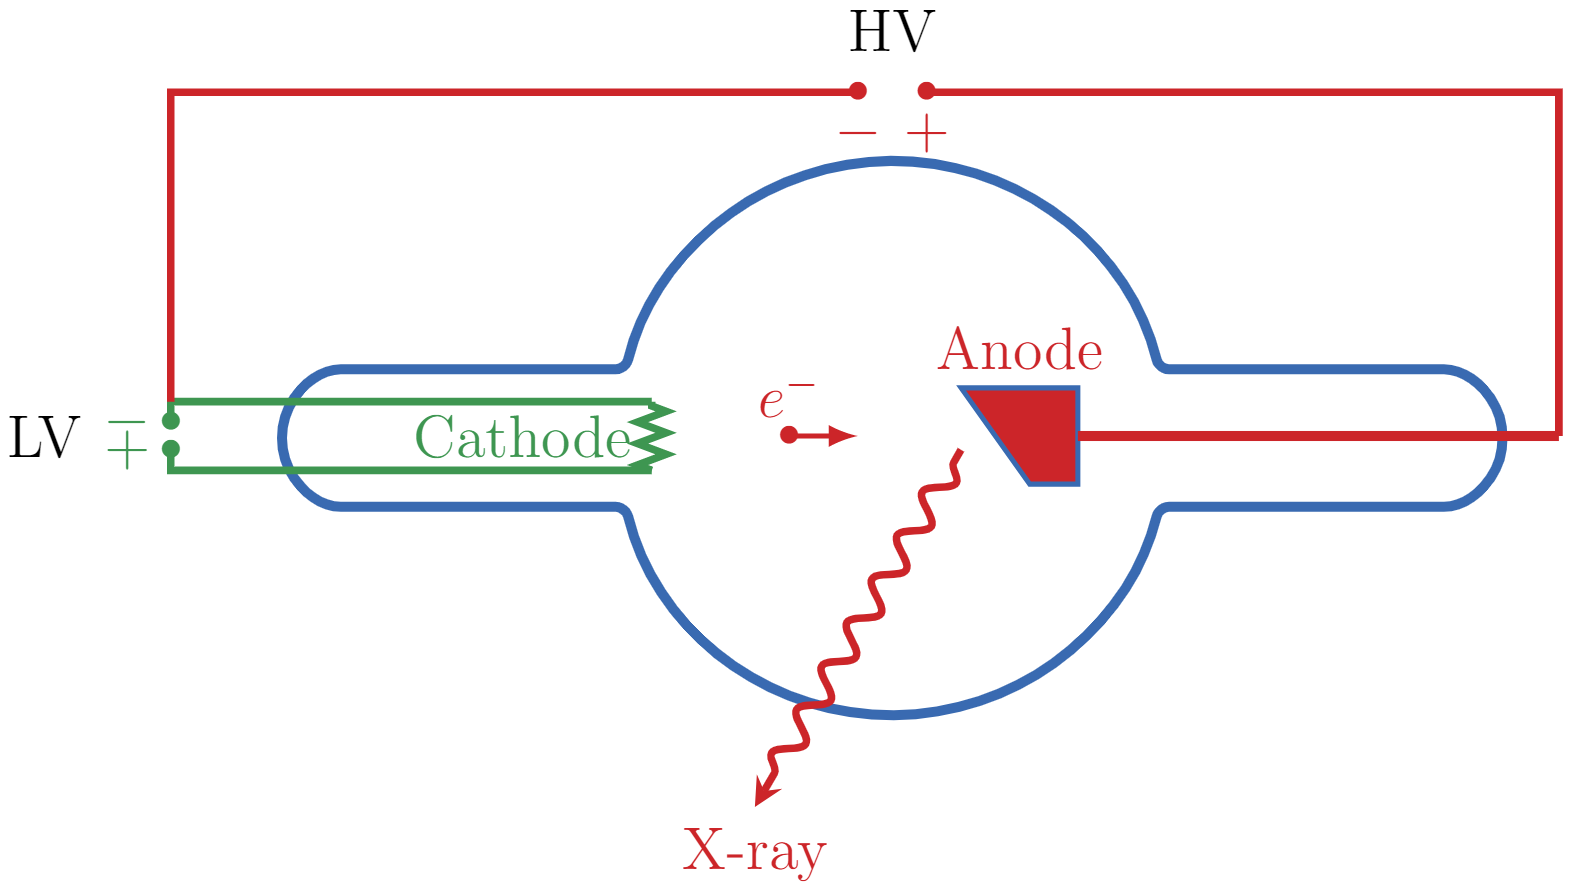
\includegraphics[width=0.7\columnwidth]{./figures/Fig6.png}
	\caption{X-ray generation process}
	\label{fig6}
\end{figure}

For more clarification, we focus on reflected x-rays. As you can see in figure \ref{fig7}, there is a 45 degrees inclination angle. For example, if you have an object at 45 degrees, you will get a reflection, and the angle between this reflection and the incidence ray is 90 degrees. With this method, you put an object and get a magnified view of it on a film.

\begin{figure}[htbp]
	%\resizebox{\linewidth}{!}{
	\centering 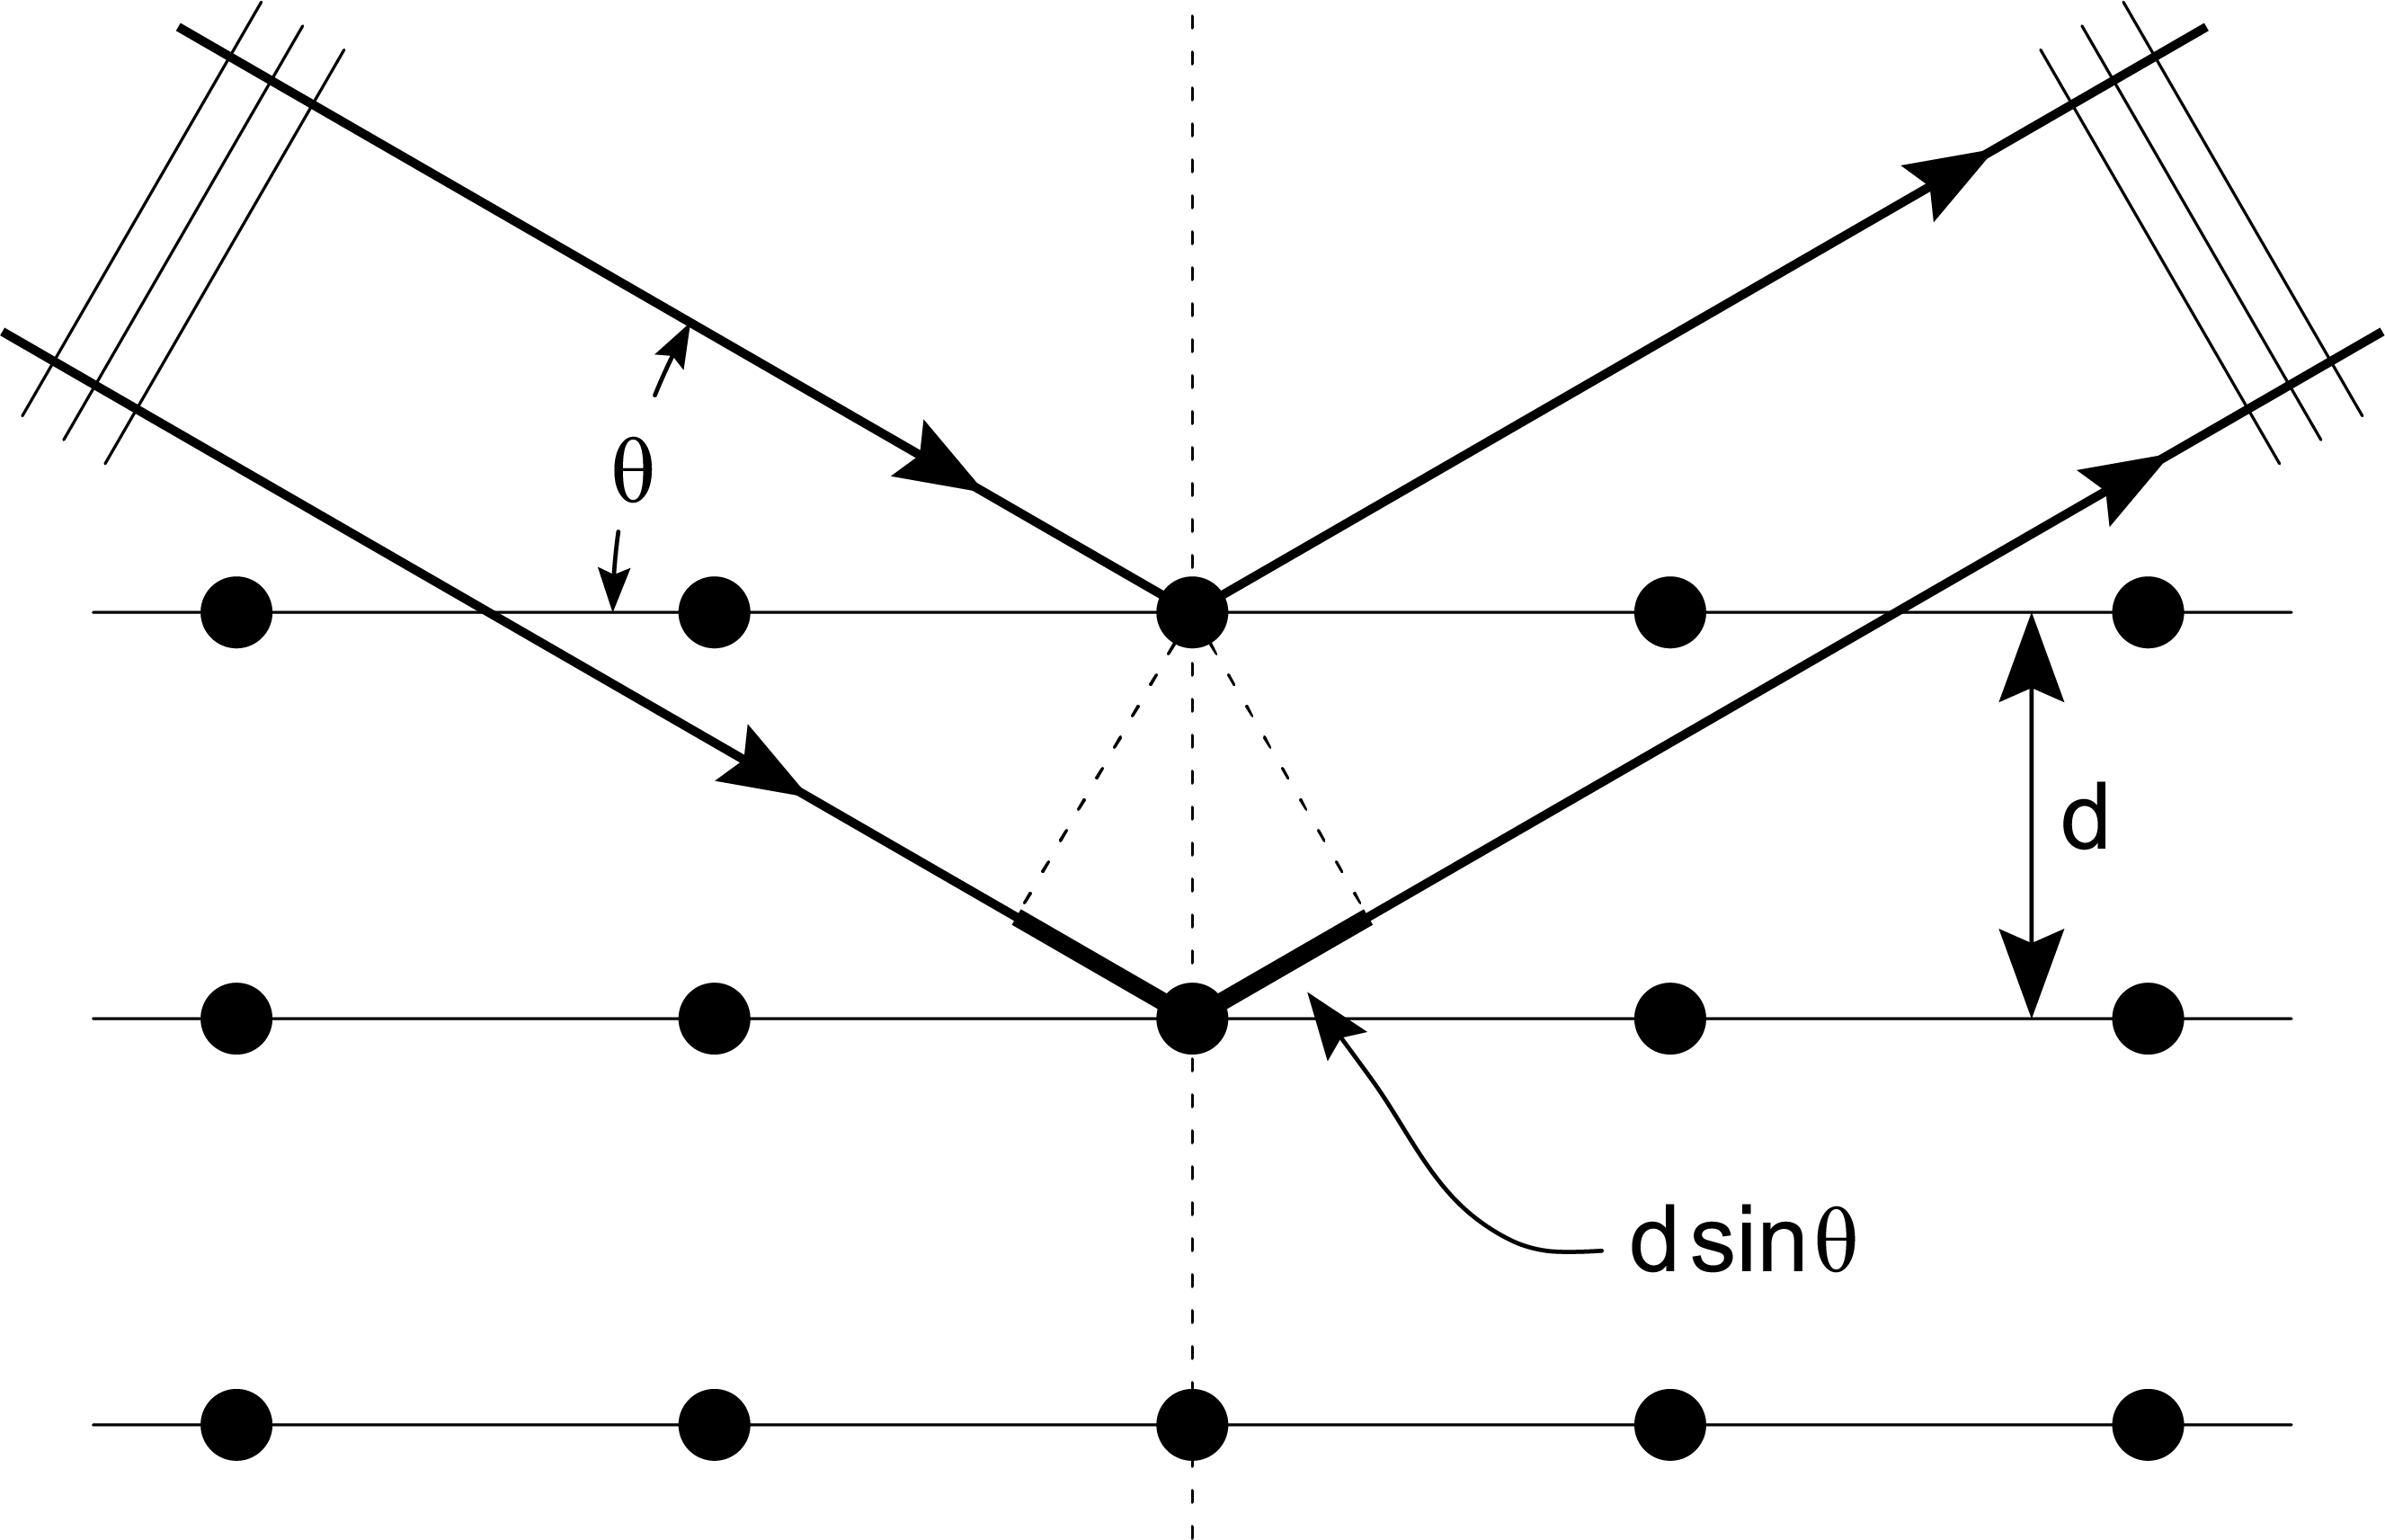
\includegraphics[width=0.7\columnwidth]{./figures/Fig7.png}
	\caption{The process of generation x-ray in more details}
	\label{fig7}
\end{figure}

The next modality is Computed Tomography, and we want to find how to acquire the images using this method. In this method, several detectors have been used, not a single one. The best way is to set an array of sensors, and each has a different line equation, to being solved out when you get the full projection. After that, you need to rotate this pair of the detector array. It keeps on rotating, and you will get multiple projections, so you can backtrack and reconstruct your whole object. Also, it is called CT reconstruction. 

In the final step, we want to find out what is a CT machine looks like. The human body is divided into three planes(x, y, and z-axis); it is three orthogonal planes in medical images. The first plane is called Coronal, which crosses from your left-hand side to the right-hand side and moves the coronal plane from front to back and vice versa. The next one is the Sagittal plane that divides your body into left and right parts, and it can moves from left to right or reverse. Finally, the other plane is called as Axial plane. This plane divides your body into top and lower parts. Figure \ref{fig8} shows a CT machine structure.

\begin{figure}[htbp]
	%\resizebox{\linewidth}{!}{
	\centering 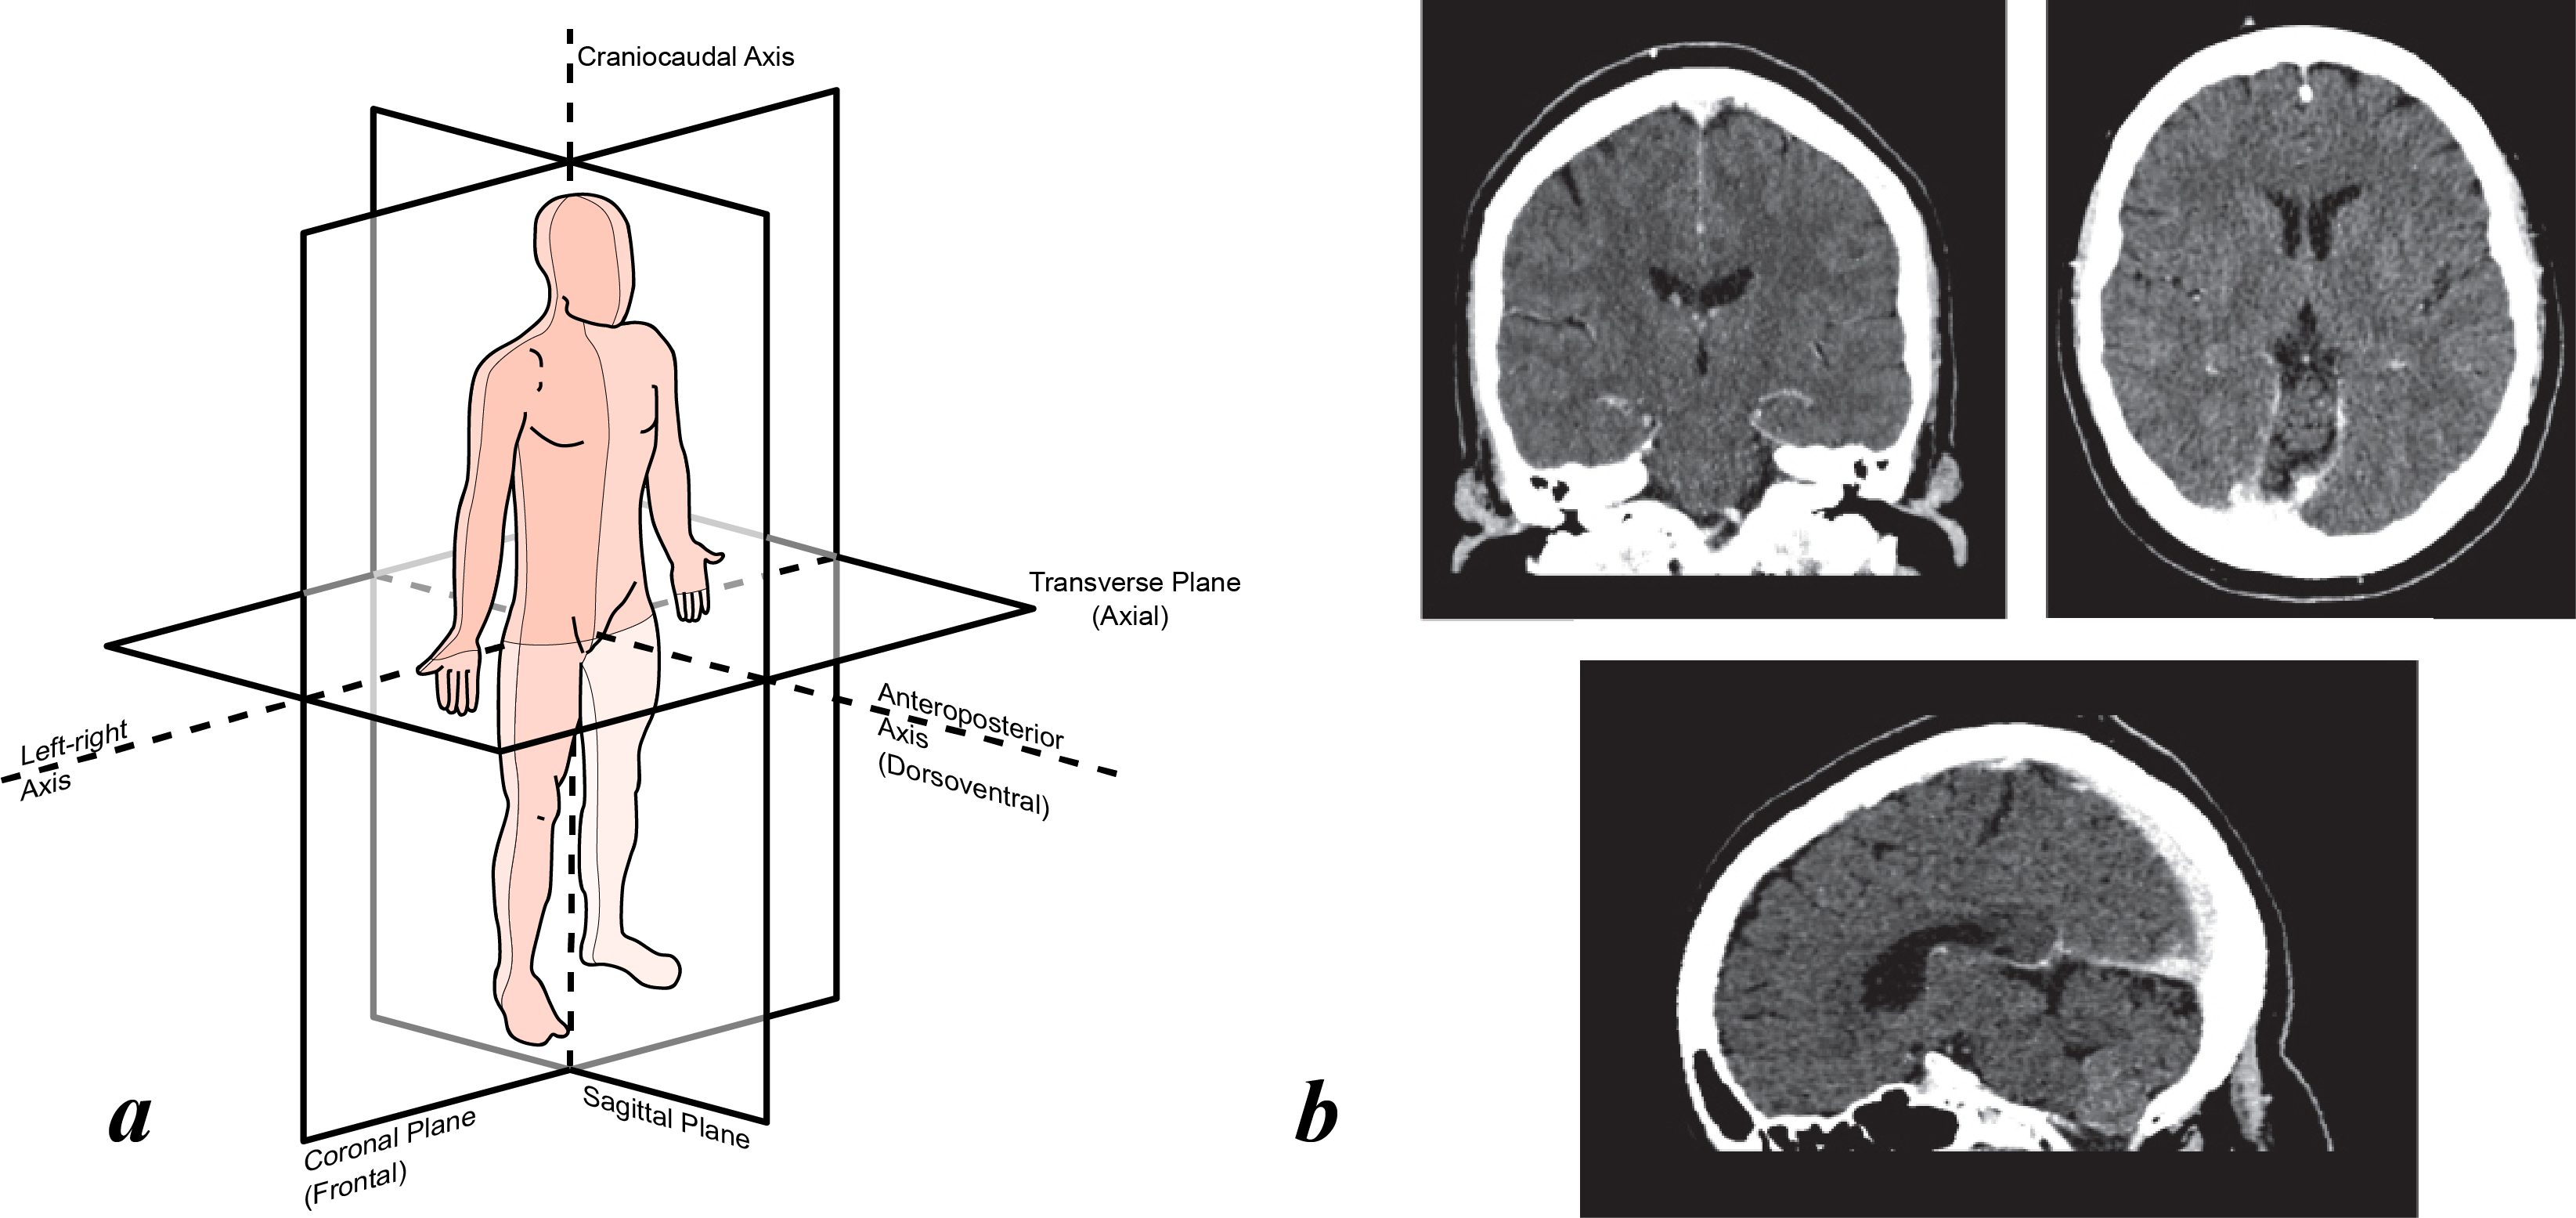
\includegraphics[width=0.85\columnwidth]{./figures/Fig8.png}
	\caption{(a) Diagram of the axial, coronal and sagittal planes. (b) Corresponding CT images of a normal brain.}
	\label{fig8}
\end{figure}


\section{Magnetic Resonance Imaging (MRI)}

The human body is made of multiple small magnets just because of the amount of water drank. This is the base of a concept known as nuclear magnetic resonance. Every single atom has a balanced ratio which is called the gyromagnetic ratio. The first part of MRI is the Spin-Echo concept. If we want to align something from a lower energy state to a higher energy state, we must provide extra energies. When we reduce the energy level, all the protons went down to a higher energy configuration. In other words, they are opposite to magnetic fields.

After some time, due to thermal motion, protons will lose some energy to other atoms. Once they keep on losing energy, they are eventually going to fall to a particular plane. Then some of them will go opposite each other, which means that the net magnetic field is 0. There are some different magnetic field directions. One of them is longitudinal; another one is traverse which is along the opposite direction. Figure \ref{fig9} illustrates these directions.

\begin{figure}[htbp]
	%\resizebox{\linewidth}{!}{
	\centering 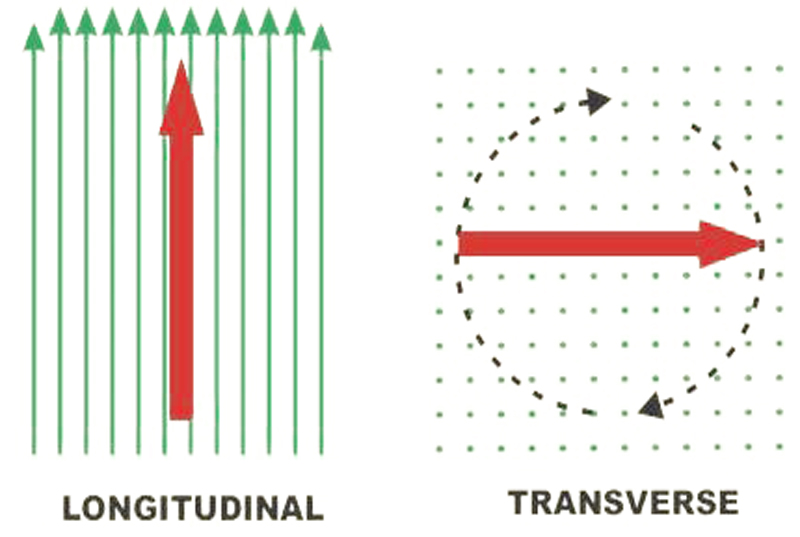
\includegraphics[width=0.55\columnwidth]{./figures/Fig9.jpg}
	\caption{Different magnetic directions}
	\label{fig9}
\end{figure}

Let’s look at different materials and their T1 and T2 relaxation time and as it shown in table \ref{tab1} the highest values are for Cerebrospinal fluids. Another interesting fact is if T1 is increasing, then T2 also is increasing. T1 is higher than fat, whereas T2 is lower than fat. Also, for muscles, T1 is higher than liver although T2 is higher than Liver but is it lower than fat. The first modality is called T1 weighed image and the second one is known as T2 weighed image.

\begin{table}[h]
	\centering
	\caption{Spin relaxation time}
	\label{tab1}
	\renewcommand{\arraystretch}{1.2}
	\begin{tabular}{|c|c|c|}
		\hline
		\textbf{Tissue}              & \textbf{T1(ms)} & \textbf{T2(ms)} \\ \hline
		Fat                 & 260             & 80              \\ \hline
		Liver               & 550             & 40              \\ \hline
		Muscle             & 870             & 45              \\ \hline
		White matter        & 780             & 90              \\ \hline
		Gray matter         & 900             & 100             \\ \hline
		Cerebrospinal fluid & 2400            & 160             \\ \hline
	\end{tabular}
\end{table}


In table \ref{tab1}, those regions with a much higher T1 relaxation time have much higher energy, respectively. If we have an MRI of a brain (Figure \ref{fig10}), it is made out of many fats. In the T1 modality, the fat regions in the brain are shown in white color, while in the T2 modality, it is a gray matter. Also, the correspondences between T1 and T2, white matter, and gray matter appear opposite to each other, and it is because of the relation between these two modalities.

\begin{figure}[htbp]
	%\resizebox{\linewidth}{!}{
	\centering 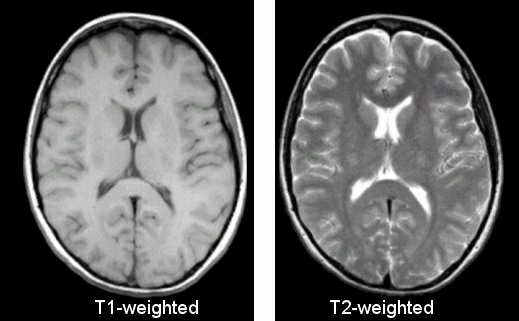
\includegraphics[width=0.5\columnwidth]{./figures/Fig10.jpg}
	\caption{T1 and T2 modalities}
	\label{fig10}
\end{figure}

The primary role of engineering comes into play when we want to apply a trick in MRI. Instead of exposing the whole body to a constant magnetic field, we create a gradient. For example, somewhere around the head, the magnetic field is about 1.5 tesla, and around the legs, it will become about 0.5 tesla. After applying this technique, we can divide the body into different slices, and each piece will have a different frequency.

Table \ref{tab2} is a quick reference for different matters in the body in T1 and T2 modalities. For example, T1 and T2 weighted images for bones or bonny-like structures (including calcifications) have an external signal. It is contrary to CT images; i.e., in CT images, bones were shown as brighter structures.

\begin{table}[htbp]
	\centering
	\caption{Comparison is made on the signal of muscles }
	\label{tab2}
	\renewcommand{\arraystretch}{1.2}
	\begin{tabular}{|c|c|c|}
		\hline
		\textbf{Tissue}            & \textbf{T1 weighted} & \textbf{T2 weighted} \\ \hline
		Bone cortex, calcification & Very low signal      & Very low signal      \\ \hline
		Bone Marrow                & High signal          & High signal          \\ \hline
		Cartilage                  & Iso signal           & Slightly low signal  \\ \hline
		Joint effusion             & Iso signal           & High signal          \\ \hline
		Acute hemorrhage           & Low to iso signal    & Low to iso signal    \\ \hline
		Subacute hemorrhage        & High signal          & High signal          \\ \hline
		Hemosiderin                & Very low signal      & Very low signal      \\ \hline
		Fat                        & High signal          & High signal          \\ \hline
	\end{tabular}
\end{table}


\section{Ultrasound Imaging}

Ultrasound is an exciting imaging modality. The prefix ultra means it is above our standard audible limit. Human ears can hear with frequencies from 20 hertz to 20-kilo hertz. In this imaging method, you have a transducer placed in exact contact on the surface; it shouldn’t have an air gap. The transducer emits a tiny bit pulse known as acoustic pulse. Actually, in ultrasound imaging, we probe waves in a fixed period and then draw the contour of all the points. It is like we throw a stone in water, and then we see circular waves around it. Figure \ref{fig11} illustrates the ultrasound mechanism.

\begin{figure}[htbp]
	%\resizebox{\linewidth}{!}{
	\centering 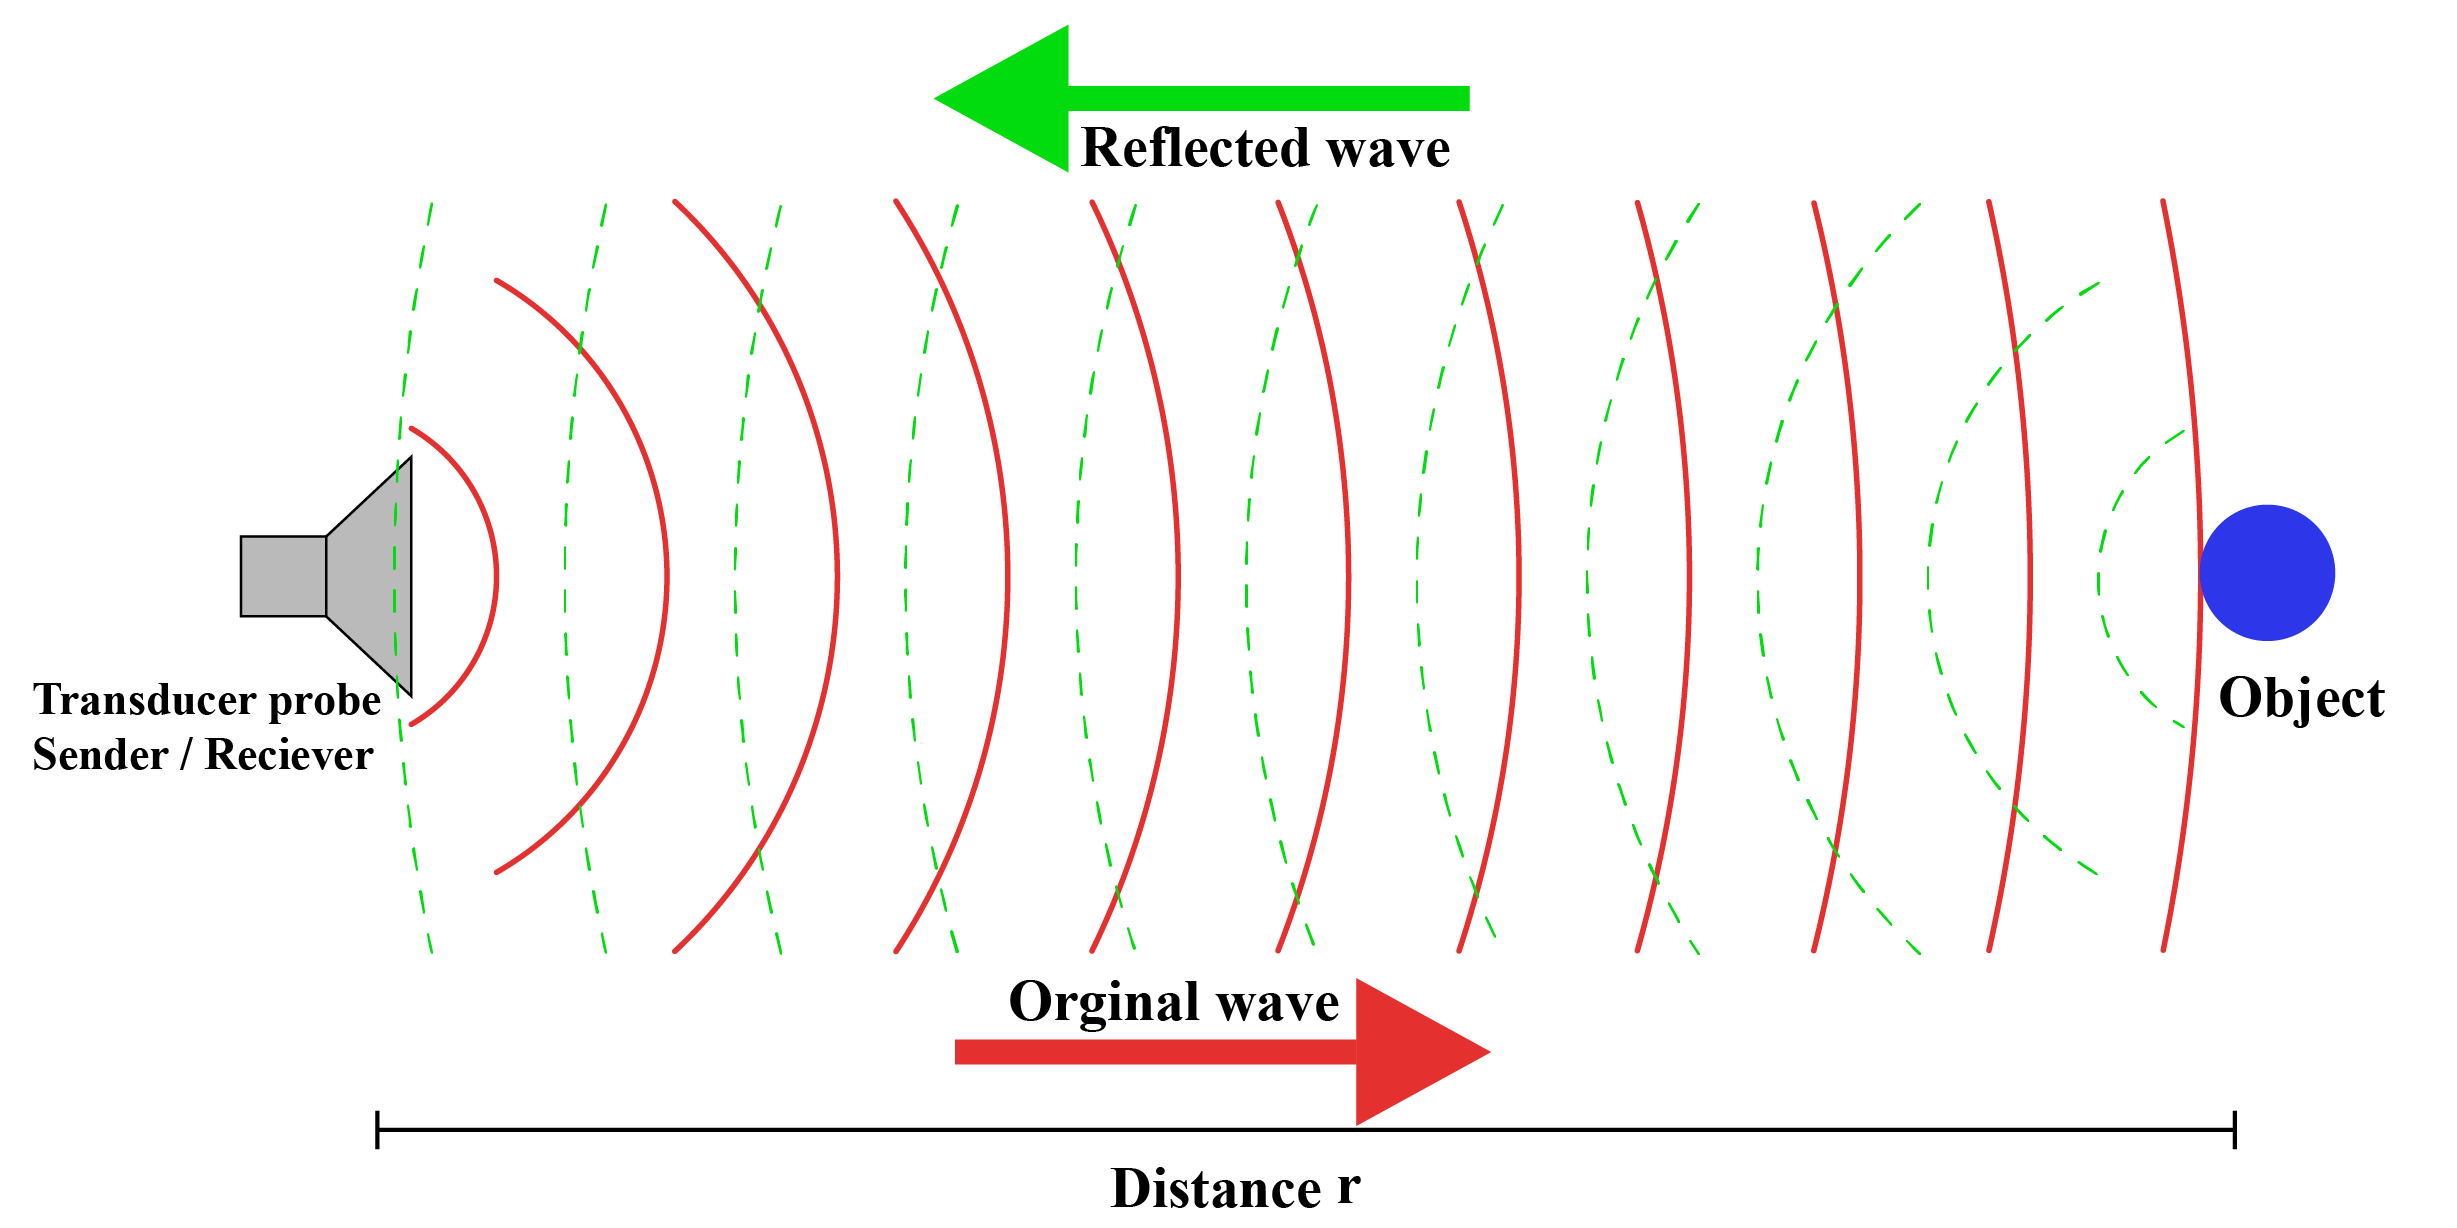
\includegraphics[width=0.7\columnwidth]{./figures/Fig11.png}
	\caption{how ultrasound works}
	\label{fig11}
\end{figure}

Interference between waves is the concept that helps to identify where the object is and what shape it is. In general, there is no control about where that object is located because, in 2d space, there is just 1d way of figuring out where the obstruction is located. The solution to this problem is to use more transducers. For example, consider we use two transducers, and they fire at the same time. The phase of the two waves is the same. Figure \ref{fig12} show this scenario. Although they come from two different sources, there is constructive interference between these two waves. So these are some points that have the highest magnitude.

\begin{figure}[htbp]
	%\resizebox{\linewidth}{!}{
	\centering 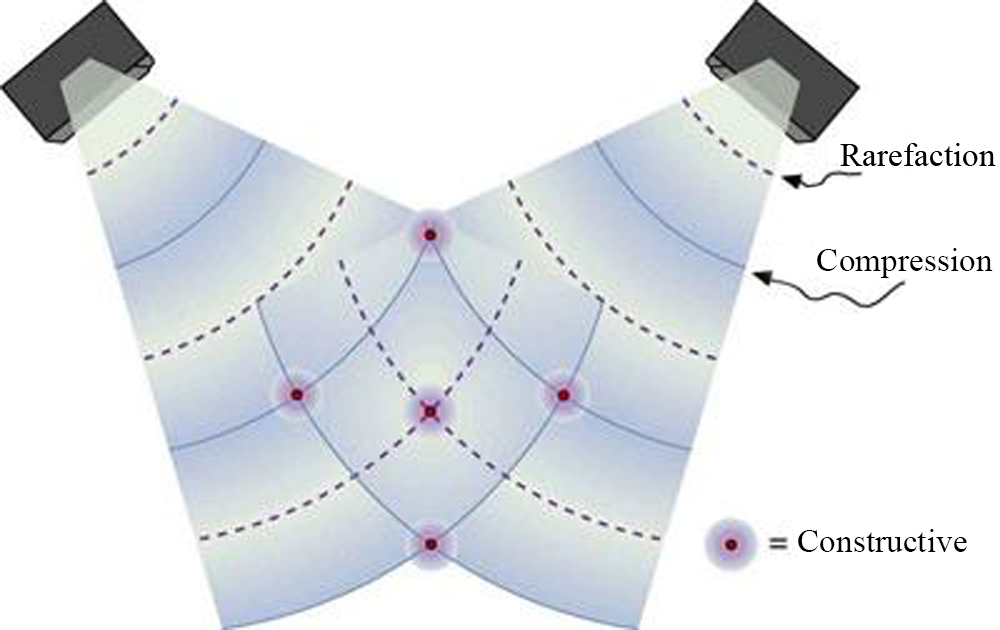
\includegraphics[width=0.7\columnwidth]{./figures/Fig12.jpg}
	\caption{how ultrasound works}
	\label{fig12}
\end{figure}

\section{Optical Microscopy and Molecular Imaging}

The last module which we cover is Optical Microscopy and Molecular imaging. The previous modules such as CT, MR, and Ultrasound are the majority of macro imaging modalities. In other words, in these modules, you look into larger parts of the body. In microscopy, you will look into a particular part of the body. This modality aims to study one single cell or a cluster of cells that was not possible with any other modalities.

A microscope usually does optical Microscopy and Molecular imaging. One of the first types of microscopy used in medical applications was the Single Photon Emission Computed Tomography (SPECT) system which was very useful to look into gamma photon generation. In this system, radio isotropy was put down along with glucose and give to the patient. If a particular organ has more glucose consumption, it means other organs are in there, and we would see more radionuclide coming down from there.

The resolution of SPECT was much lower and did not give a very high structural resolution. So, generally, structural scan systems are used either a structural CT or structural MR along with a SPECT. These multiple images are registered together to diagnose by knowing the structure and the function.

The other type of microscopy is Positron Emission Tomography, and when there is a positron emitted, you would see a pair of gamma photons created; this means that we always need to have a pair of detectors that are 180 degrees apart and if these detectors rotate we will be sensing a pair of incidences. This method helps to reduce noise, and the noises on each detector are independent. Figure \ref{fig13} shows this method. 

\begin{figure}[htbp]
	%\resizebox{\linewidth}{!}{
	\centering 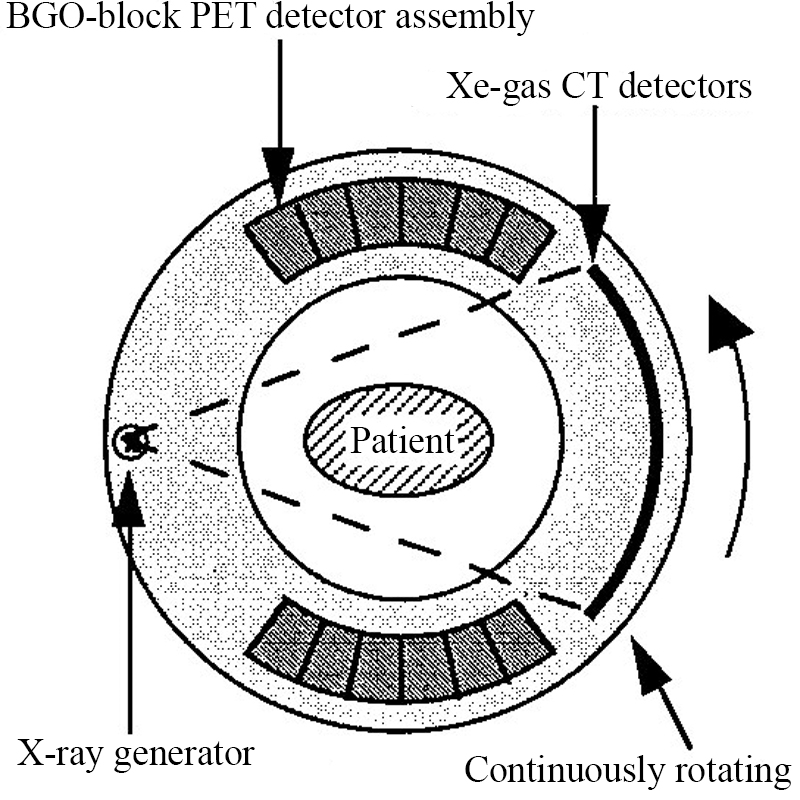
\includegraphics[width=0.7\columnwidth]{./figures/Fig13.jpg}
	\caption{Optical PET imaging instrument}
	\label{fig13}
\end{figure}

